\section{Observations}
	We carried out the experiment under two different conditions: 
	
	\begin{enumerate}
		\item Indoors in presence of incandescent lamp
		\item In presence of sunlight
	\end{enumerate}
	All the curves have been fitted with equation:
	
	\begin{equation}
		I(V) = Ae^{BV} - C.
		\label{eq:2}
	\end{equation}
	
	Here, $A$, $B$, and $C$ are the parameters. The I-V Characteristics of the solar cell under those conditions are as follows:
	\subsection{Indoors in presence of Incandescent lamp}
		\begin{table}[H]
	\centering
	\resizebox{\columnwidth}{!}{%
	\begin{tabular}{|cc|cc|cc|cc|cc|}
		\hline
		\multicolumn{2}{|c|}{\textbf{White}} & \multicolumn{2}{c|}{\textbf{Pink}} & \multicolumn{2}{c|}{\textbf{Green}} & \multicolumn{2}{c|}{\textbf{Red}} & \multicolumn{2}{c|}{\textbf{Yellow}}                                                                                                                                             \\ \hline
		\multicolumn{1}{|c|}{\textbf{V}}     & \textbf{$I\;(\mu A)$}              & \multicolumn{1}{c|}{\textbf{V}}     & \textbf{$I\;(\mu A)$}             & \multicolumn{1}{c|}{\textbf{V}}      & \textbf{$I\;(\mu A)$} & \multicolumn{1}{c|}{\textbf{V}} & \textbf{$I\;(\mu A)$} & \multicolumn{1}{c|}{\textbf{V}} & \textbf{$I\;(\mu A)$} \\ \hline
		\multicolumn{1}{|c|}{0.88}           & 10.6                               & \multicolumn{1}{c|}{0.731}          & 7                                 & \multicolumn{1}{c|}{0.521}           & 2                     & \multicolumn{1}{c|}{0.553}      & 27                    & \multicolumn{1}{c|}{0.715}      & 21                    \\ \hline
		\multicolumn{1}{|c|}{0.843}          & 143.2                              & \multicolumn{1}{c|}{0.696}          & 91                                & \multicolumn{1}{c|}{0.481}           & 26                    & \multicolumn{1}{c|}{0.513}      & 80                    & \multicolumn{1}{c|}{0.675}      & 119                   \\ \hline
		\multicolumn{1}{|c|}{0.81}           & 259.5                              & \multicolumn{1}{c|}{0.661}          & 145                               & \multicolumn{1}{c|}{0.441}           & 69                    & \multicolumn{1}{c|}{0.475}      & 116                   & \multicolumn{1}{c|}{0.634}      & 244                   \\ \hline
		\multicolumn{1}{|c|}{0.762}          & 381.5                              & \multicolumn{1}{c|}{0.626}          & 211                               & \multicolumn{1}{c|}{0.402}           & 86                    & \multicolumn{1}{c|}{0.436}      & 156                   & \multicolumn{1}{c|}{0.593}      & 312                   \\ \hline
		\multicolumn{1}{|c|}{0.693}          & 560                                & \multicolumn{1}{c|}{0.591}          & 218                               & \multicolumn{1}{c|}{0.361}           & 121                   & \multicolumn{1}{c|}{0.398}      & 169                   & \multicolumn{1}{c|}{0.554}      & 431                   \\ \hline
		\multicolumn{1}{|c|}{0.615}          & 693                                & \multicolumn{1}{c|}{0.556}          & 292                               & \multicolumn{1}{c|}{0.322}           & 145                   & \multicolumn{1}{c|}{0.360}      & 193                   & \multicolumn{1}{c|}{0.513}      & 485                   \\ \hline
		\multicolumn{1}{|c|}{0.579}          & 737                                & \multicolumn{1}{c|}{0.521}          & 332                               & \multicolumn{1}{c|}{0.282}           & 176                   & \multicolumn{1}{c|}{0.320}      & 240                   & \multicolumn{1}{c|}{0.472}      & 541                   \\ \hline
		\multicolumn{1}{|c|}{0.53}           & 773                                & \multicolumn{1}{c|}{0.486}          & 388                               & \multicolumn{1}{c|}{0.242}           & 201                   & \multicolumn{1}{c|}{0.281}      & 248                   & \multicolumn{1}{c|}{0.432}      & 560                   \\ \hline
		\multicolumn{1}{|c|}{0.5}            & 829                                & \multicolumn{1}{c|}{0.450}          & 418                               & \multicolumn{1}{c|}{0.202}           & 198                   & \multicolumn{1}{c|}{0.243}      & 283                   & \multicolumn{1}{c|}{0.39}       & 651                   \\ \hline
		\multicolumn{1}{|c|}{0.473}          & 856                                & \multicolumn{1}{c|}{0.415}          & 460                               & \multicolumn{1}{c|}{0.162}           & 211                   & \multicolumn{1}{c|}{0.204}      & 285                   & \multicolumn{1}{c|}{0.35}       & 674                   \\ \hline
		\multicolumn{1}{|c|}{0.425}          & 896                                & \multicolumn{1}{c|}{0.380}          & 502                               & \multicolumn{1}{c|}{0.124}           & 246                   & \multicolumn{1}{c|}{0.166}      & 294                   & \multicolumn{1}{c|}{0.31}       & 759                   \\ \hline
		\multicolumn{1}{|c|}{0.388}          & 923                                & \multicolumn{1}{c|}{0.345}          & 554                               & \multicolumn{1}{c|}{0.082}           & 243                   & \multicolumn{1}{c|}{0.128}      & 313                   & \multicolumn{1}{c|}{0.27}       & 710                   \\ \hline
		\multicolumn{1}{|c|}{0.3}            & 939                                & \multicolumn{1}{c|}{0.310}          & 589                               & \multicolumn{1}{c|}{0.044}           & 280                   & \multicolumn{1}{c|}{0.089}      & 318                   & \multicolumn{1}{c|}{0.229}      & 777                   \\ \hline
		\multicolumn{1}{|c|}{0.284}          & 941                                & \multicolumn{1}{c|}{0.275}          & 592                               & \multicolumn{1}{c|}{}                &                       & \multicolumn{1}{c|}{0.049}      & 342                   & \multicolumn{1}{c|}{0.19}       & 798                   \\ \hline
		\multicolumn{1}{|c|}{0.261}          & 942                                & \multicolumn{1}{c|}{0.240}          & 620                               & \multicolumn{1}{c|}{}                &                       & \multicolumn{1}{c|}{}           &                       & \multicolumn{1}{c|}{0.148}      & 822                   \\ \hline
		\multicolumn{1}{|c|}{0.22}           & 943                                & \multicolumn{1}{c|}{0.205}          & 596                               & \multicolumn{1}{c|}{}                &                       & \multicolumn{1}{c|}{}           &                       & \multicolumn{1}{c|}{0.107}      & 831                   \\ \hline
		\multicolumn{1}{|c|}{0.204}          & 944                                & \multicolumn{1}{c|}{0.170}          & 637                               & \multicolumn{1}{c|}{}                &                       & \multicolumn{1}{c|}{}           &                       & \multicolumn{1}{c|}{}           &                       \\ \hline
		\multicolumn{1}{|c|}{0.18}           & 945                                & \multicolumn{1}{c|}{}               &                                   & \multicolumn{1}{c|}{}                &                       & \multicolumn{1}{c|}{}           &                       & \multicolumn{1}{c|}{}           &                       \\ \hline
		\multicolumn{1}{|c|}{0.168}          & 945                                & \multicolumn{1}{c|}{}               &                                   & \multicolumn{1}{c|}{}                &                       & \multicolumn{1}{c|}{}           &                       & \multicolumn{1}{c|}{}           &                       \\ \hline
	\end{tabular}%
	}
	\caption{Data indoors in the presence of an incandescent lamp}
	\label{tab:indoor}
\end{table}

		The data collected for the I-V characteristics of the solar cell under incandescent lamp is given in \hyperref[tab:indoor]{Table 1}. The I-V curve for no filter has been shown in \hyperref[graph:1]{Figure 5} and the I-V curve for different filters has been shown in \hyperref[graph:2]{Figure 6}.

		\begin{figure}[H]
			\centering
			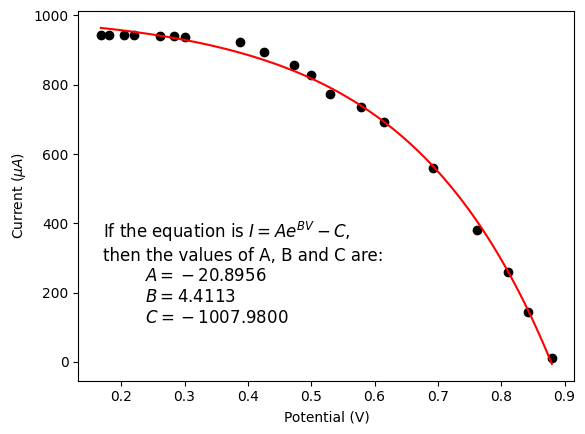
\includegraphics[width=0.75\columnwidth]{images/graph_1.png}
			\caption{I vs V curve for solar filter under white light indoors}
			\label{graph:1}
		\end{figure}

		\begin{figure}[H]
			\centering
			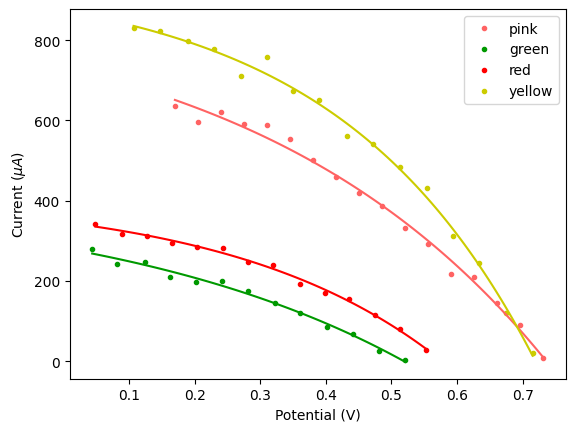
\includegraphics[width=0.75\columnwidth]{images/graph_2.png}
			\caption{I-V curve for data with different filters indoors}
			\label{graph:2}
		\end{figure}

	\subsection{Outdoors in presence of Sunlight}
		\begin{table}[H]
	\centering
	\begin{tabular}{|cc|cc|cc|cc|cc|}
		\hline
		\multicolumn{2}{|c|}{\textbf{White}} & \multicolumn{2}{c|}{\textbf{Pink}} & \multicolumn{2}{c|}{\textbf{Green}} & \multicolumn{2}{c|}{\textbf{Red}} & \multicolumn{2}{c|}{\textbf{Yellow}}                                                                                                                                             \\ \hline
		\multicolumn{1}{|c|}{\textbf{V}}     & \textbf{$I\;(\mu A)$}              & \multicolumn{1}{c|}{\textbf{V}}     & \textbf{$I\;(\mu A)$}             & \multicolumn{1}{c|}{\textbf{V}}      & \textbf{$I\;(\mu A)$} & \multicolumn{1}{c|}{\textbf{V}} & \textbf{$I\;(\mu A)$} & \multicolumn{1}{c|}{\textbf{V}} & \textbf{$I\;(\mu A)$} \\ \hline
		\multicolumn{1}{|c|}{1.531}          & 12                                 & \multicolumn{1}{c|}{1.53}           & 2                                 & \multicolumn{1}{c|}{1.494}           & 10                    & \multicolumn{1}{c|}{1.540}      & 9                     & \multicolumn{1}{c|}{1.540}      & 1                     \\ \hline
		\multicolumn{1}{|c|}{1.475}          & 78                                 & \multicolumn{1}{c|}{1.494}          & 23                                & \multicolumn{1}{c|}{1.445}           & 45                    & \multicolumn{1}{c|}{1.491}      & 35                    & \multicolumn{1}{c|}{1.457}      & 70                    \\ \hline
		\multicolumn{1}{|c|}{1.420}          & 113                                & \multicolumn{1}{c|}{1.445}          & 46                                & \multicolumn{1}{c|}{1.395}           & 62                    & \multicolumn{1}{c|}{1.441}      & 72                    & \multicolumn{1}{c|}{1.372}      & 113                   \\ \hline
		\multicolumn{1}{|c|}{1.365}          & 138                                & \multicolumn{1}{c|}{1.395}          & 64                                & \multicolumn{1}{c|}{1.346}           & 76                    & \multicolumn{1}{c|}{1.392}      & 90                    & \multicolumn{1}{c|}{1.290}      & 133                   \\ \hline
		\multicolumn{1}{|c|}{1.309}          & 146                                & \multicolumn{1}{c|}{1.346}          & 82                                & \multicolumn{1}{c|}{1.296}           & 87                    & \multicolumn{1}{c|}{1.343}      & 104                   & \multicolumn{1}{c|}{1.207}      & 149                   \\ \hline
		\multicolumn{1}{|c|}{1.254}          & 158                                & \multicolumn{1}{c|}{1.296}          & 95                                & \multicolumn{1}{c|}{1.246}           & 95                    & \multicolumn{1}{c|}{1.293}      & 112                   & \multicolumn{1}{c|}{1.123}      & 160                   \\ \hline
		\multicolumn{1}{|c|}{1.198}          & 170                                & \multicolumn{1}{c|}{1.246}          & 110                               & \multicolumn{1}{c|}{1.197}           & 96                    & \multicolumn{1}{c|}{1.244}      & 131                   & \multicolumn{1}{c|}{1.038}      & 162                   \\ \hline
		\multicolumn{1}{|c|}{1.143}          & 164                                & \multicolumn{1}{c|}{1.197}          & 120                               & \multicolumn{1}{c|}{1.147}           & 96                    & \multicolumn{1}{c|}{1.195}      & 137                   & \multicolumn{1}{c|}{0.955}      & 163                   \\ \hline
		\multicolumn{1}{|c|}{1.087}          & 169                                & \multicolumn{1}{c|}{1.147}          & 131                               & \multicolumn{1}{c|}{1.098}           & 98                    & \multicolumn{1}{c|}{1.145}      & 144                   & \multicolumn{1}{c|}{0.873}      & 164                   \\ \hline
		\multicolumn{1}{|c|}{1.031}          & 178                                & \multicolumn{1}{c|}{1.098}          & 145                               & \multicolumn{1}{c|}{1.048}           & 102                   & \multicolumn{1}{c|}{1.096}      & 150                   & \multicolumn{1}{c|}{0.788}      & 165                   \\ \hline
		\multicolumn{1}{|c|}{0.976}          & 174                                & \multicolumn{1}{c|}{1.048}          & 151                               & \multicolumn{1}{c|}{0.998}           & 105                   & \multicolumn{1}{c|}{1.047}      & 155                   & \multicolumn{1}{c|}{0.703}      & 164                   \\ \hline
		\multicolumn{1}{|c|}{0.921}          & 182                                & \multicolumn{1}{c|}{0.998}          & 156                               & \multicolumn{1}{c|}{0.949}           & 106                   & \multicolumn{1}{c|}{0.997}      & 157                   & \multicolumn{1}{c|}{0.620}      & 170                   \\ \hline
		\multicolumn{1}{|c|}{0.865}          & 191                                & \multicolumn{1}{c|}{0.949}          & 158                               & \multicolumn{1}{c|}{0.899}           & 107                   & \multicolumn{1}{c|}{0.948}      & 160                   & \multicolumn{1}{c|}{0.539}      & 168                   \\ \hline
		\multicolumn{1}{|c|}{0.810}          & 184                                & \multicolumn{1}{c|}{0.899}          & 165                               & \multicolumn{1}{c|}{0.850}           & 108                   & \multicolumn{1}{c|}{0.899}      & 162                   & \multicolumn{1}{c|}{}           &                       \\ \hline
		\multicolumn{1}{|c|}{0.754}          & 182                                & \multicolumn{1}{c|}{0.850}          & 174                               & \multicolumn{1}{c|}{0.800}           & 108                   & \multicolumn{1}{c|}{0.849}      & 162                   & \multicolumn{1}{c|}{}           &                       \\ \hline
		\multicolumn{1}{|c|}{0.698}          & 198                                & \multicolumn{1}{c|}{0.800}          & 176                               & \multicolumn{1}{c|}{}                &                       & \multicolumn{1}{c|}{0.800}      & 163                   & \multicolumn{1}{c|}{}           &                       \\ \hline
		\multicolumn{1}{|c|}{0.643}          & 189                                & \multicolumn{1}{c|}{}               &                                   & \multicolumn{1}{c|}{}                &                       & \multicolumn{1}{c|}{}           &                       & \multicolumn{1}{c|}{}           &                       \\ \hline
	\end{tabular}
	\caption{Data outdoors in the presence of Sun}
	\label{tab:outdoor}
\end{table}

		The data collected for the I-V characteristics of the solar cell under incandescent lamp is given in \hyperref[tab:outdoor]{Table 2}. The I-V curve for no filter has been shown in \hyperref[graph:3]{Figure 7} and the I-V curve for different filters has been shown in \hyperref[graph:4]{Figure 8}.

		\begin{figure}[h]
			\centering
			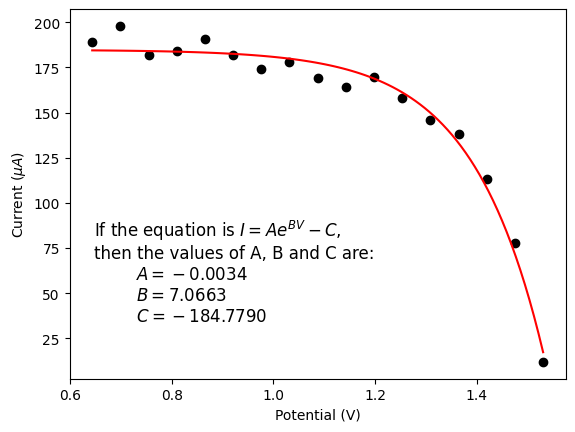
\includegraphics[width=0.75\columnwidth]{images/graph_3.png}
			\caption{I vs V curve for solar filter under white light outdoors}
			\label{graph:3}
		\end{figure}

		\begin{figure}[h]
			\centering
			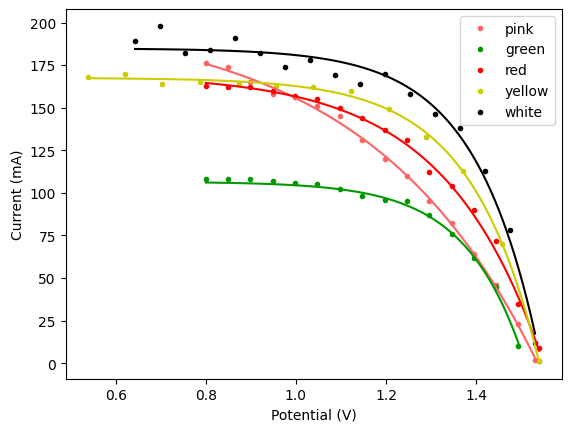
\includegraphics[width=0.75\columnwidth]{images/graph_4.png}
			\caption{I-V curve for data with different filters outdoors}
			\label{graph:4}
		\end{figure}
